% Created 2020-09-01 Tue 11:40
% Intended LaTeX compiler: pdflatex
\documentclass[presentation]{beamer}
\usepackage[utf8]{inputenc}
\usepackage[T1]{fontenc}
\usepackage{graphicx}
\usepackage{grffile}
\usepackage{longtable}
\usepackage{wrapfig}
\usepackage{rotating}
\usepackage[normalem]{ulem}
\usepackage{amsmath}
\usepackage{textcomp}
\usepackage{amssymb}
\usepackage{capt-of}
\usepackage{hyperref}
\usetheme{UoB}
\author{Mark Blyth}
\date{\textit{[2020-08-31 Mon]}}
\title{Stuff going wrong}
\hypersetup{
 pdfauthor={Mark Blyth},
 pdftitle={Stuff going wrong},
 pdfkeywords={},
 pdfsubject={},
 pdfcreator={Emacs 27.1 (Org mode 9.3)}, 
 pdflang={English}}
\begin{document}

\maketitle


\section{Background}
\label{sec:org254367c}
\begin{frame}[label={sec:org5417e82}]{Week's work}
\begin{itemize}
\item Finished draft of conference paper
\begin{itemize}
\item Too long
\end{itemize}
\end{itemize}
\vfill
\begin{itemize}
\item Worked on splines in CBC
\begin{itemize}
\item Doesn't work
\end{itemize}
\end{itemize}
\vfill
\begin{itemize}
\item Started re-writing conference paper
\begin{itemize}
\item No splines discretisation
\item Struggling to motivate why the work is valuable
\end{itemize}
\end{itemize}
\end{frame}

\section{Paper}
\label{sec:org58a6983}
\begin{frame}[label={sec:org1e5168f}]{Paper}
\begin{itemize}
\item Abstract focuses on cleaning noise from signals with surrogate modelling
\item Paper draft 1 covers surrogate filtering, and splines discretisation
\end{itemize}
\vfill      
Issues:
\begin{itemize}
\item Paper is too long
\begin{itemize}
\item 17 pages, instead of 10
\item Could trim it, but can't trim 7 pages out without removing key content
\end{itemize}
\item Splines doesn't work
\begin{itemize}
\item I don't want to publish about splines until I know they do what I claim
\end{itemize}
\item Don't have enough time to both trim paper, and fix splines
\end{itemize}
\end{frame}

\begin{frame}[label={sec:orgd26bc96}]{Proposed plan}
\begin{itemize}
\item Remove discretisation from paper
\begin{itemize}
\item Make paper all about cleaning signals up with surrogates, as discussed in abstract
\item Most realistic goal for getting paper done by deadline
\item Issue: I'm not convinced surrogates are very useful
\end{itemize}
\end{itemize}

\vfill
\begin{itemize}
\item Try to get splines to work
\begin{itemize}
\item Write separate conference paper on splines discretisation?
\item Will have the time to demonstrate the method working
\end{itemize}
\end{itemize}
\end{frame}

\section{Splines}
\label{sec:orga3bafbf}
\begin{frame}[label={sec:org1c16163}]{Splines in CBC}
\begin{itemize}
\item Took working Fourier/Duffing, substituted Fourier for splines
\begin{itemize}
\item Doesn't work
\end{itemize}
\end{itemize}
\vfill
\begin{itemize}
\item IO-Map method
\begin{itemize}
\item IO-map maps control-target to system output
\item Fixed-point of IO-map means control target = system output
\item Proportional control means fixed-points are noninvasive
\end{itemize}
\end{itemize}
\vfill
\begin{itemize}
\item Continuation procedure solves for input = output
\end{itemize}
\end{frame}

\begin{frame}[label={sec:org1ecc7e2}]{Step 1}
\begin{center}
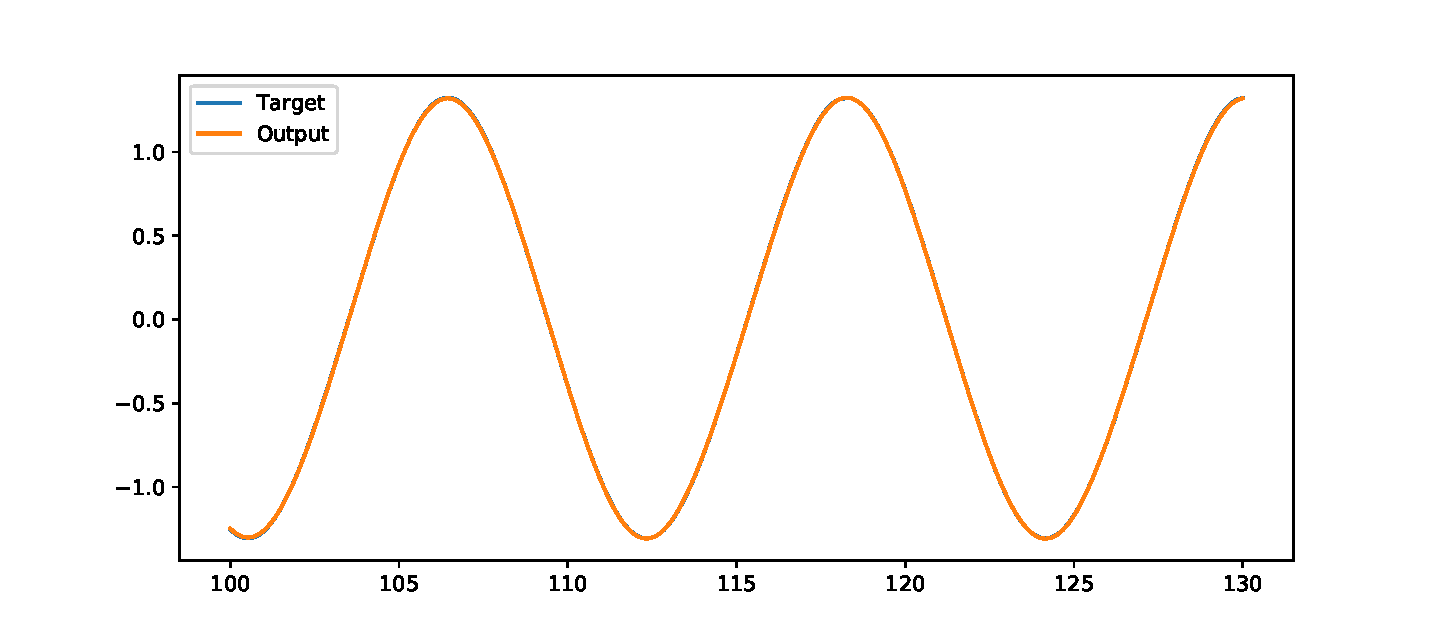
\includegraphics[width=.9\linewidth]{./step1.pdf}
\end{center}
\end{frame}
\begin{frame}[label={sec:org1a82c13}]{Step 2}
\begin{center}
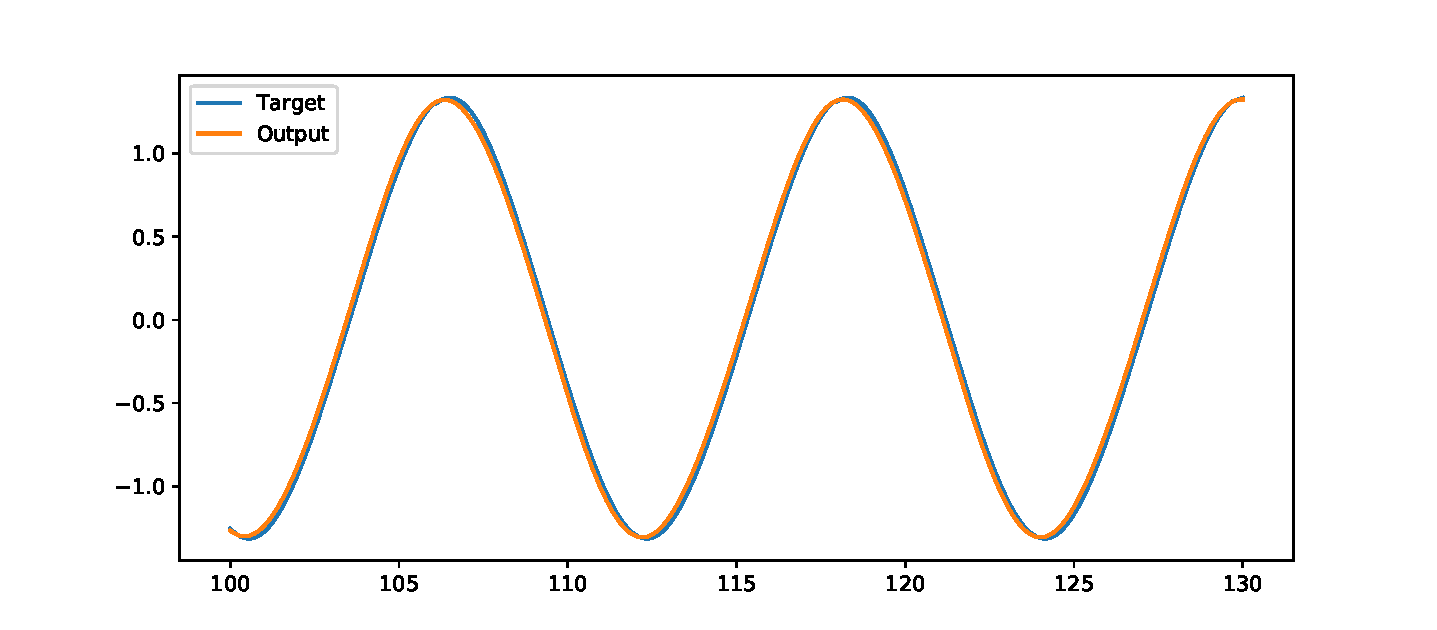
\includegraphics[width=.9\linewidth]{./step2.pdf}
\end{center}
\end{frame}
\begin{frame}[label={sec:org1d1371d}]{Step 3}
\begin{center}
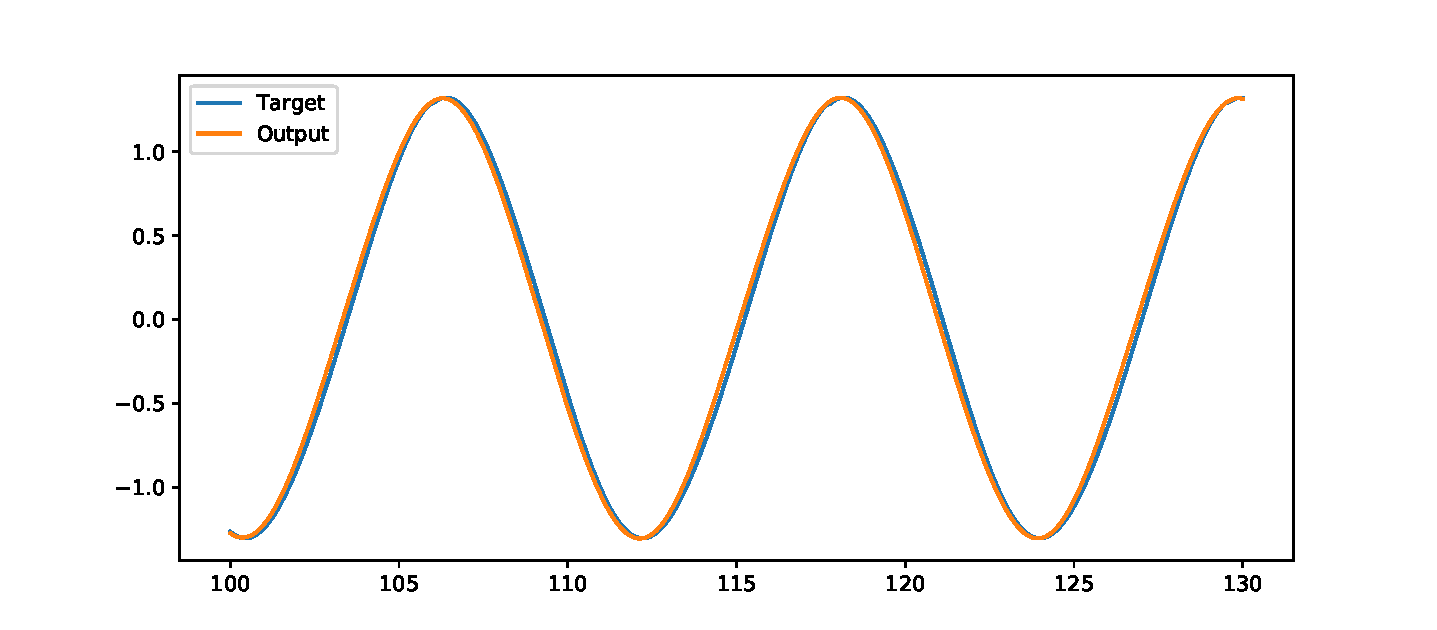
\includegraphics[width=.9\linewidth]{./step3.pdf}
\end{center}
\end{frame}
\begin{frame}[label={sec:orgd86f374}]{Step 4}
\begin{center}
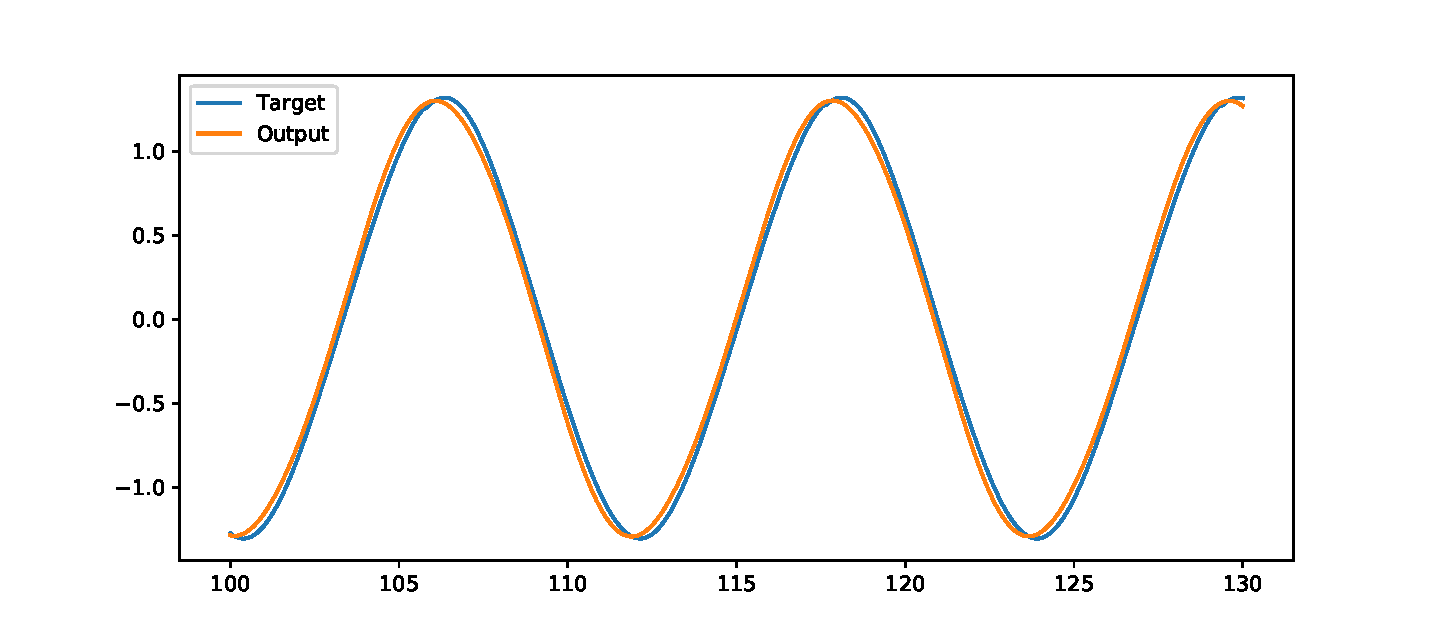
\includegraphics[width=.9\linewidth]{./step4.pdf}
\end{center}
\end{frame}
\begin{frame}[label={sec:orgd95f12a}]{Step 5}
\begin{center}
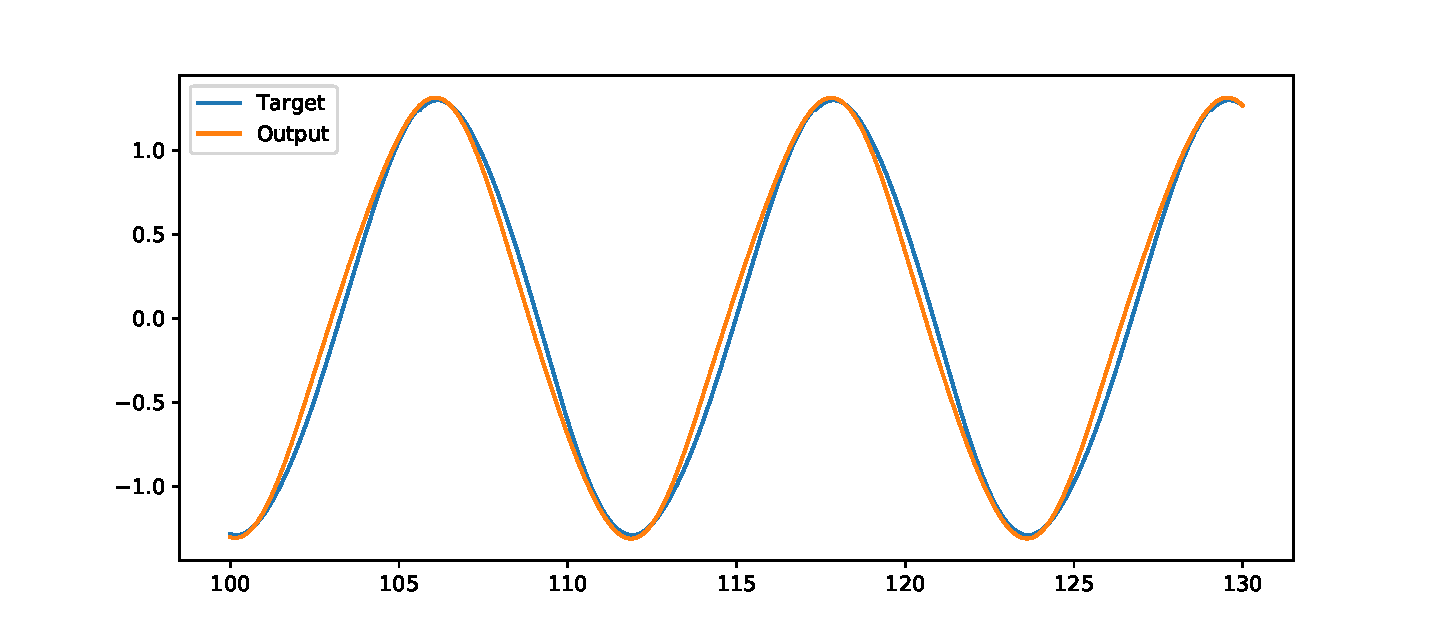
\includegraphics[width=.9\linewidth]{./step5.pdf}
\end{center}
\end{frame}
\begin{frame}[label={sec:org3f77254}]{Step 6}
\begin{center}
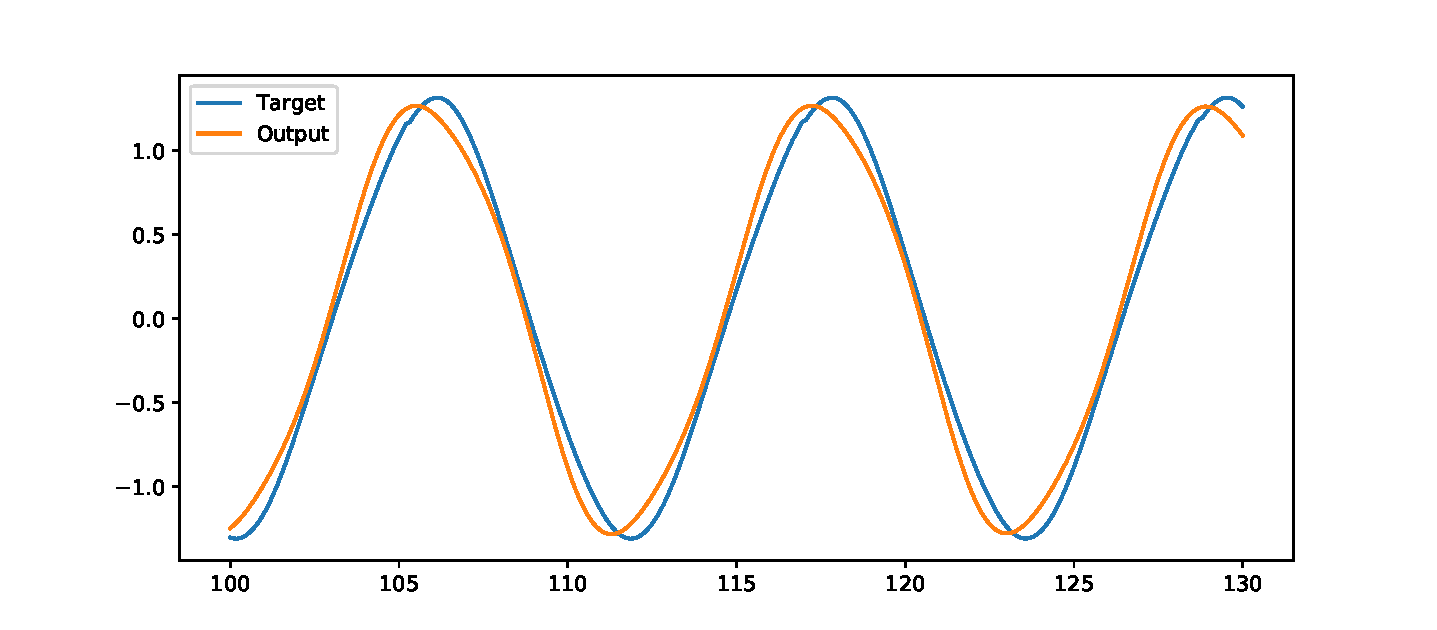
\includegraphics[width=.9\linewidth]{./step6.pdf}
\end{center}
\end{frame}
\begin{frame}[label={sec:org082e0c6}]{Step 7}
\begin{center}
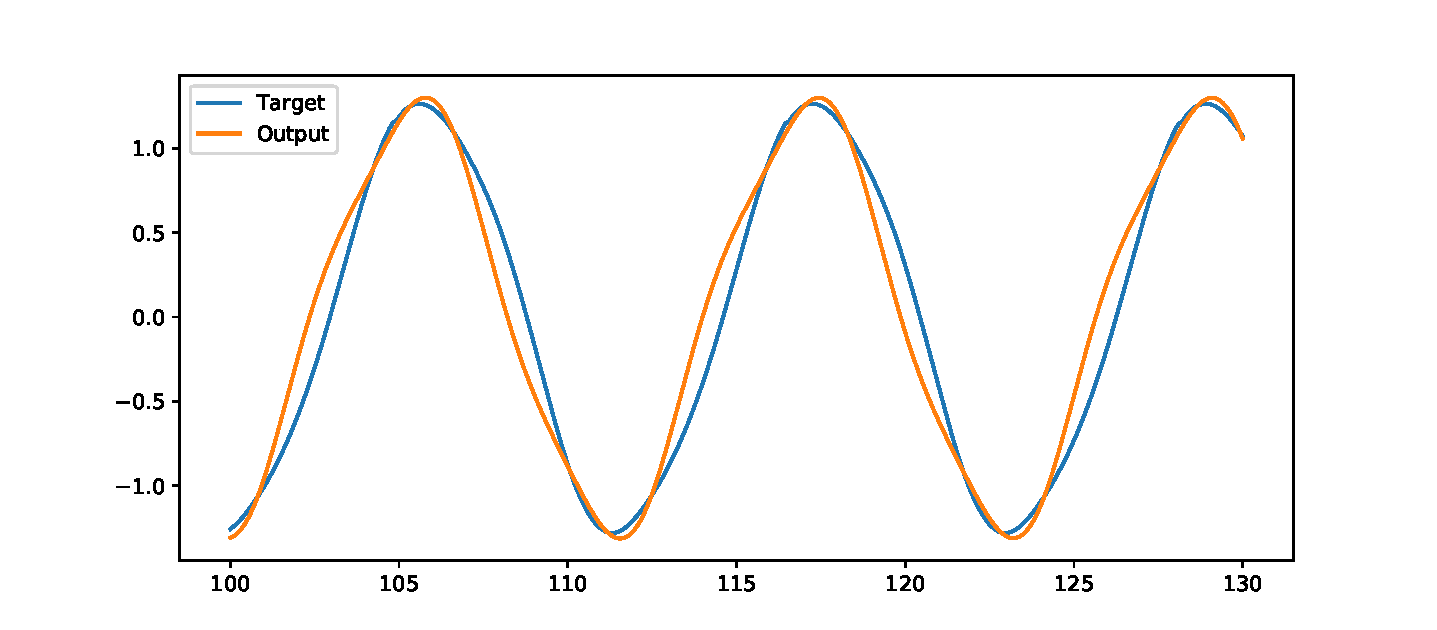
\includegraphics[width=.9\linewidth]{./step7.pdf}
\end{center}
\end{frame}
\begin{frame}[label={sec:org4249204}]{Step 8}
\begin{center}
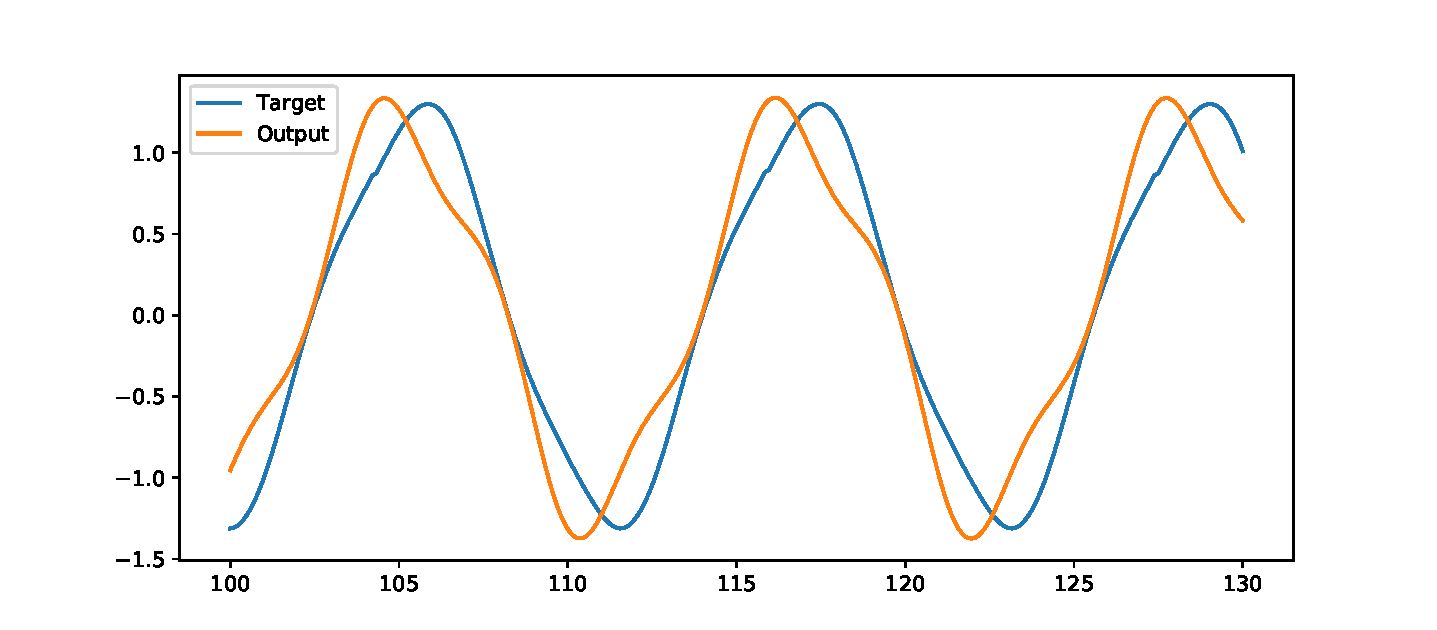
\includegraphics[width=.9\linewidth]{./step8.pdf}
\end{center}
\end{frame}
\begin{frame}[label={sec:org28aa33d}]{Step 9}
\begin{center}
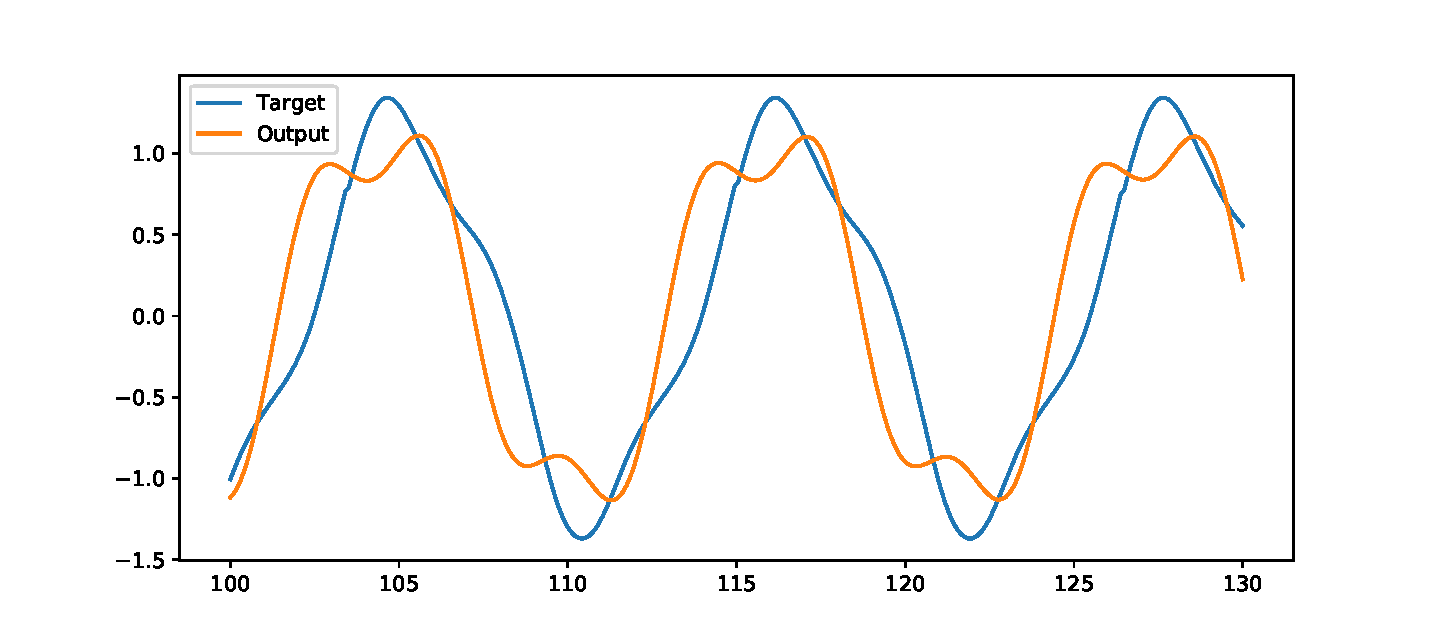
\includegraphics[width=.9\linewidth]{./step9.pdf}
\end{center}
\end{frame}
\begin{frame}[label={sec:org66cd61e}]{Step 10}
\begin{center}
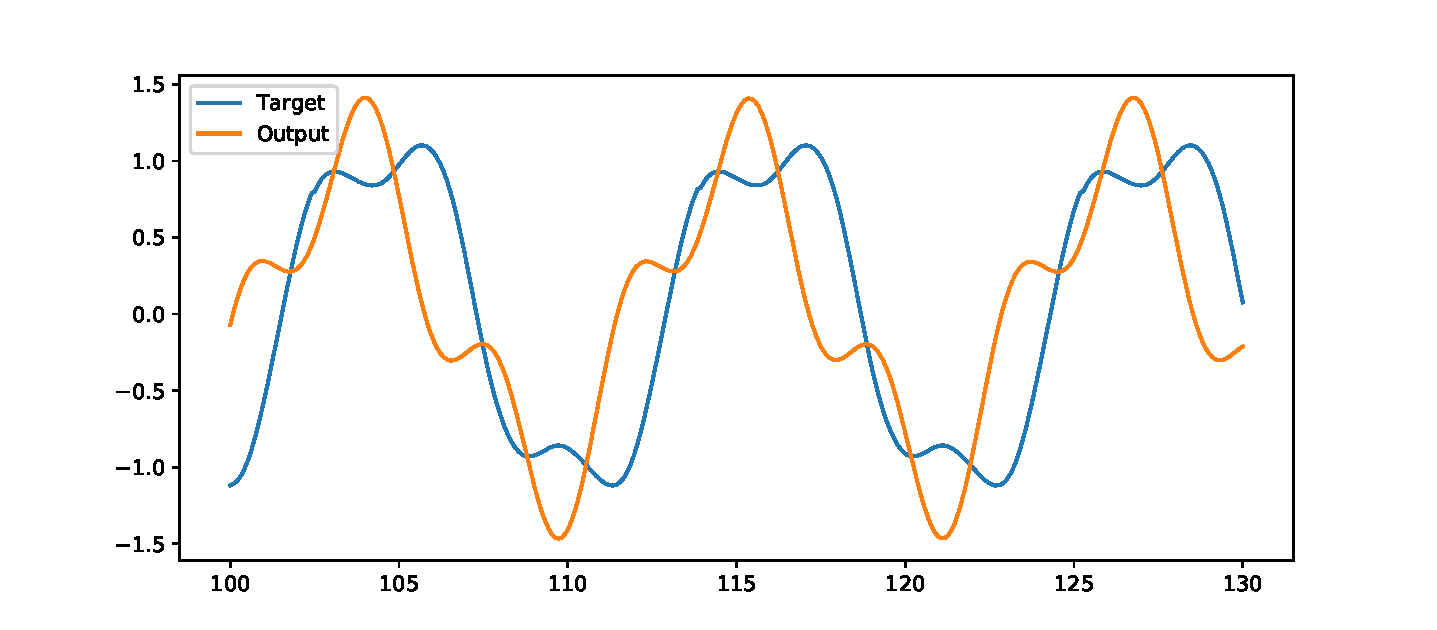
\includegraphics[width=.9\linewidth]{./step10.pdf}
\end{center}
\end{frame}

\begin{frame}[label={sec:orgc6e83aa}]{Setup}
\begin{itemize}
\item \(K_p=1\)
\begin{itemize}
\item Worked for Fourier/Duffing
\item Increasing causes CBC to fail faster
\end{itemize}
\item Solver = Levenberg-Marquardt algo
\begin{itemize}
\item Most numerically stable; others fail within one or two steps
\end{itemize}
\item Evenly-spaced knots
\begin{itemize}
\item Optimized knots fail even faster
\end{itemize}
\item 10 knots
\begin{itemize}
\item No change using more / fewer knots
\end{itemize}
\item Default solver tolerance
\begin{itemize}
\item Lower = faster failure
\end{itemize}
\end{itemize}

No idea why things aren't working
\end{frame}

\section{Surrogates}
\label{sec:org69e31a0}
\begin{frame}[label={sec:org9f0dfdc}]{Surrogates paper}
\begin{itemize}
\item Using few Fourier harmonics doesn't fit `difficult' signals
\end{itemize}
\vfill
\begin{itemize}
\item Using many Fourier harmonics doesn't average out noise
\end{itemize}
\vfill
\begin{itemize}
\item Surrogates can be used to filter out noise, for better discretisation
\begin{itemize}
\item No phase shift or signal distortion
\end{itemize}
\end{itemize}
\end{frame}

\begin{frame}[label={sec:org9a589b5}]{Surrogates}
Direct Fourier; too few harmonics to fully fit the signal

\begin{center}
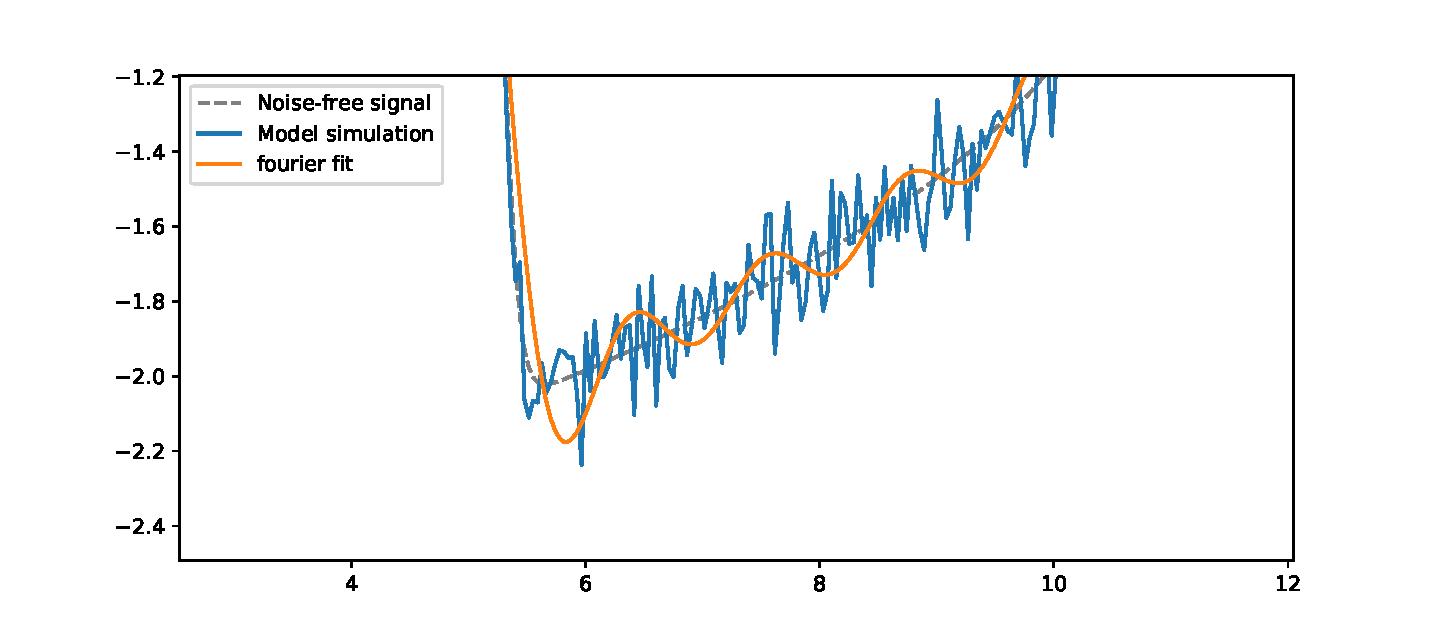
\includegraphics[width=.9\linewidth]{./needs_more.pdf}
\end{center}
\end{frame}

\begin{frame}[label={sec:orgb4e23d4}]{Surrogates}
Direct Fourier; enough harmonics to fit the signal, but also noise

\begin{center}
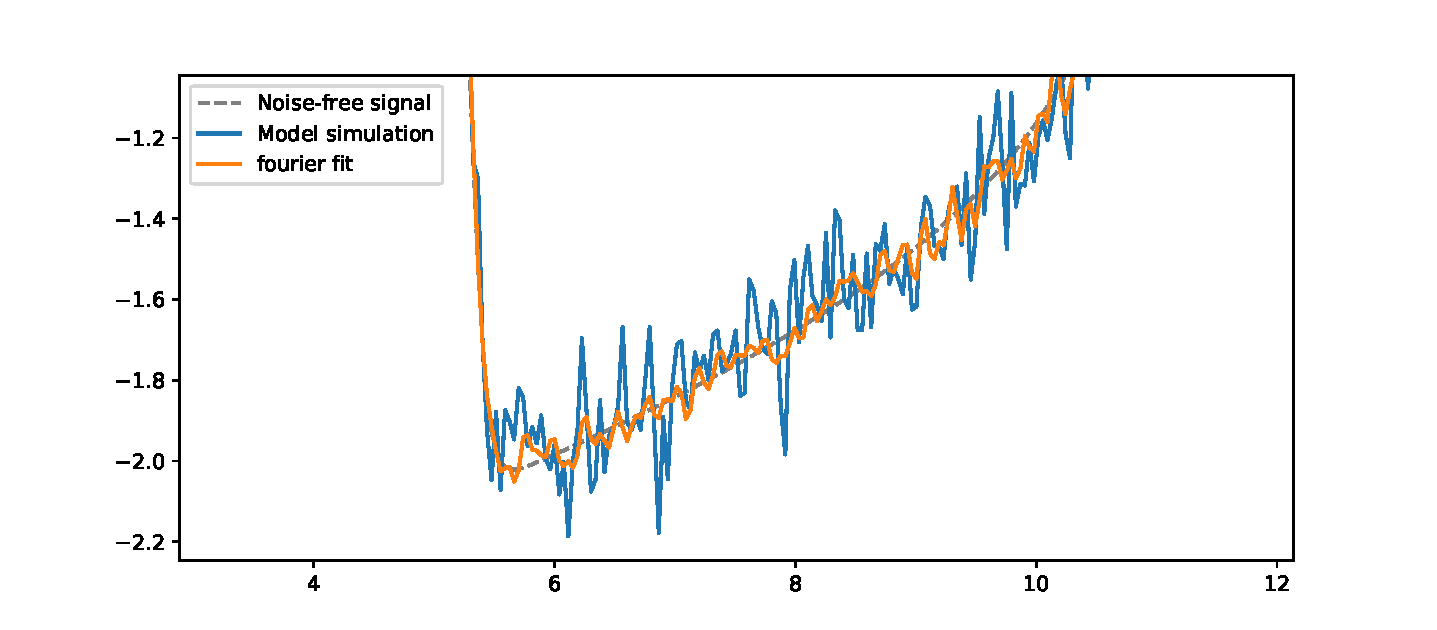
\includegraphics[width=.9\linewidth]{./fits_noise.pdf}
\end{center}
\end{frame}

\begin{frame}[label={sec:orgcf640fc}]{Surrogates}
Splines surrogate model; noise is removed, so Fourier can be fitted accurately

\begin{center}
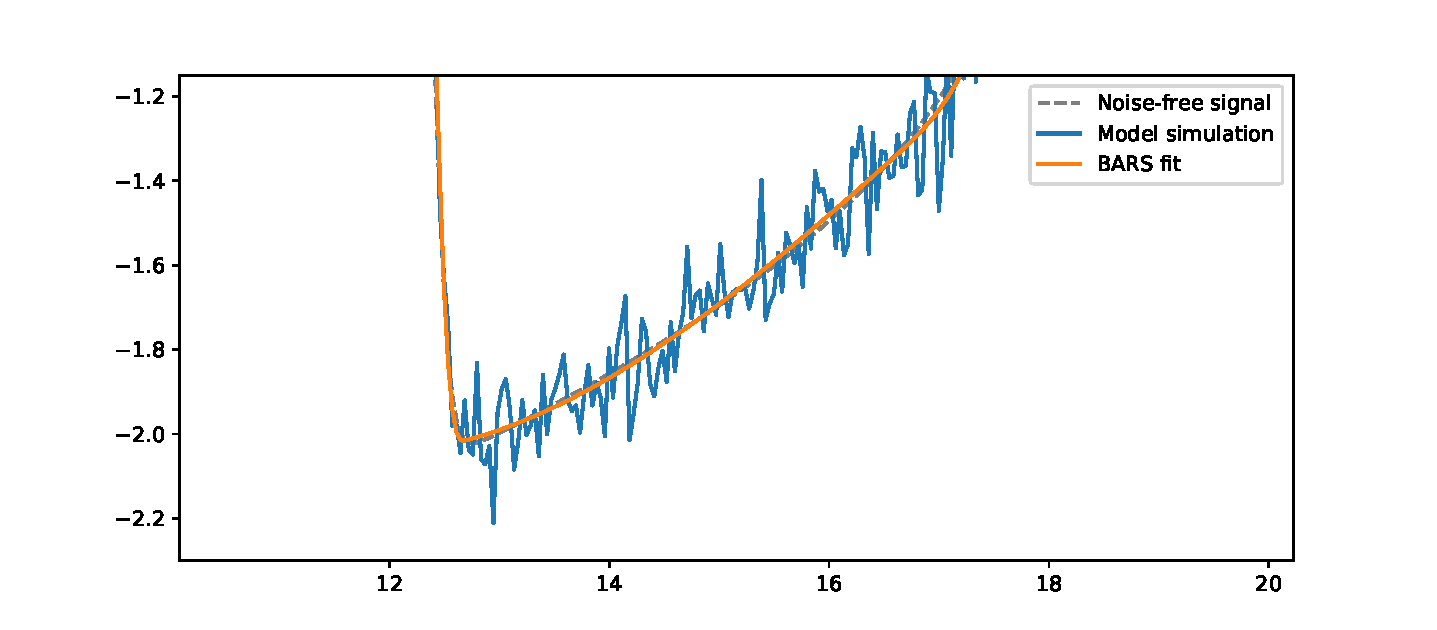
\includegraphics[width=.9\linewidth]{./barsd.pdf}
\end{center}
\end{frame}
\begin{frame}[label={sec:org75f01d8}]{Choosing number of harmonics}
Idea: quantify model noisiness by a curvature measure
\vfill

\begin{itemize}
\item \(c_i = h^{-2}(x_{i-1} - 2x_i + x_{i+1})\)
\begin{itemize}
\item Finite differences pointwise-curvature approximation
\end{itemize}
\end{itemize}
\vfill
\begin{itemize}
\item Majority of curvatures \emph{should} be small
\begin{itemize}
\item Median pointwise-curvature is a good statistic for model noisiness
\end{itemize}
\end{itemize}
\vfill
\begin{itemize}
\item How do curvature, error change with number of harmonics?
\begin{itemize}
\item Low curvature, high MSPE = too few harmonics
\item High curvature, low MSPE = too many harmonics
\item Optimal harmonics = low curvature, low MSPE
\end{itemize}
\end{itemize}
\end{frame}

\begin{frame}[label={sec:org227842d}]{Finding the sweetspot}
\begin{center}
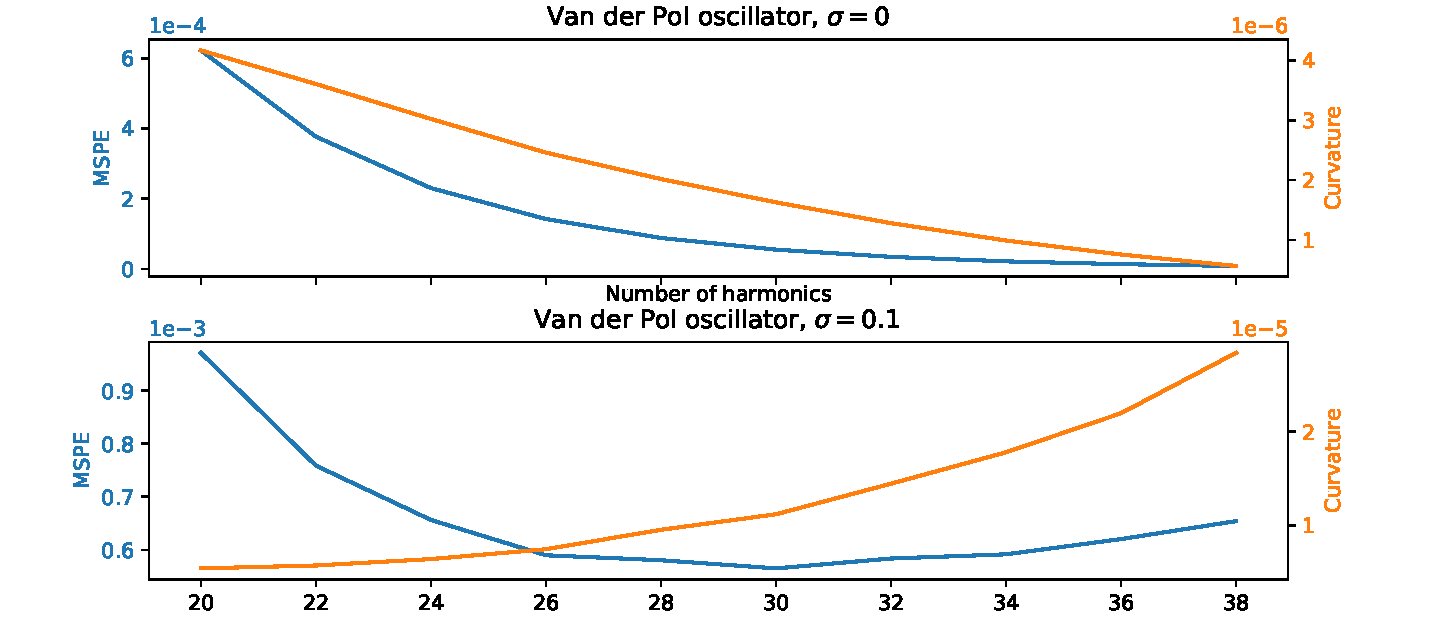
\includegraphics[width=.9\linewidth]{./sweetspot1.pdf}
\end{center}
\end{frame}

\begin{frame}[label={sec:orgbd3270e}]{Good enough?}
\begin{center}
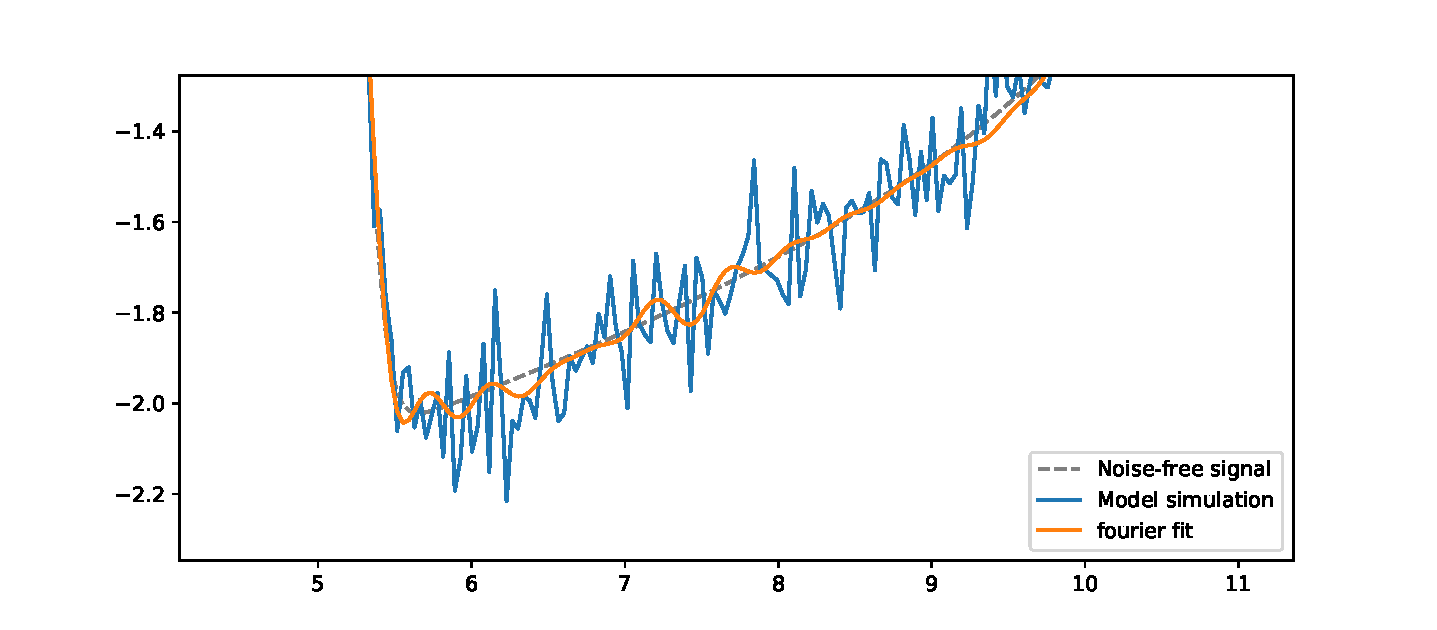
\includegraphics[width=.9\linewidth]{./fourier_sweetspot.pdf}
\end{center}
\end{frame}

\begin{frame}[label={sec:org4fd1b21}]{Issues}
\begin{itemize}
\item Surrogates do clean up the signal, but is the improvement really enough to be worthwhile?
\begin{itemize}
\item \alert{According to MSPE, surrogates and Fourier perform equally well}
\end{itemize}
\end{itemize}
\vfill
\begin{itemize}
\item Is anyone really going to harmonically force a multiple-timescale system?
\begin{itemize}
\item Fourier filters effectively when there's few harmonics, so surrogate filtering becomes unnecessary
\item Surrogate filtering appears to be useful when we have many harmonics, but in these cases we'd use a more efficient discretisation
\item The splines discretisors are noise-robust, so surrogates become unnecessary
\end{itemize}
\end{itemize}
\end{frame}

\begin{frame}[label={sec:org3cfff39}]{Are surrogates worth publishing?}
\begin{itemize}
\item Fixes a problem that doesn't really exist
\begin{itemize}
\item Not useful for few-harmonics-signals, as Fourier filters noise out
\item Not useful for many-harmonics-signals, as we would do better using a novel discretisation
\end{itemize}
\end{itemize}
\vfill
\begin{itemize}
\item Even when surrogates do work, the resulting improvement is minimal
\end{itemize}
\vfill
\begin{itemize}
\item Hard to write about surrogates being useful when prediction errors are worse than raw Fourier
\begin{itemize}
\item Hard to quantitatively demonstrate that surrogates do anything
\end{itemize}
\end{itemize}
\end{frame}

\section{Next steps}
\label{sec:orgef3ff29}
\begin{frame}[label={sec:org3413f9f}]{Next steps}
\begin{itemize}
\item Keep (re)writing conference paper?
\begin{itemize}
\item My opinion: cancel it, spend the time on discretisation
\end{itemize}
\end{itemize}
\vfill
\begin{itemize}
\item Keep working on splines, once paper is done
\begin{itemize}
\item Try to understand and fix their lack of numerical stability
\item Demonstrate on \emph{in silico} CBC
\begin{itemize}
\item IO map method and `other' method
\end{itemize}
\end{itemize}
\end{itemize}
\end{frame}
\end{document}
